\begin{minipage}{0.45\textwidth}
    \centering
    \[
    \tanh(x) = 2\sigma(2x) - 1 = \frac{e^x - e^{-x}}{e^x + e^{-x}}
    \]
\end{minipage}
\hfill
\begin{minipage}{0.45\textwidth}
    \centering
    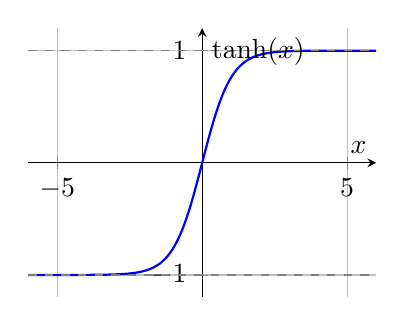
\begin{tikzpicture}[scale=1]
        \begin{axis}[
            xlabel=$x$,
            ylabel=$\tanh(x)$,
            grid=major,
            axis lines=middle,
            xmin=-6, xmax=6,
            ymin=-1.2, ymax=1.2,
            samples=200,
            width=6cm,
            height=5cm
        ]
            \addplot[blue, thick, domain=-6:6] {tanh(x)};
            \addplot[dashed, gray] coordinates {(-6,1) (6,1)};
            \addplot[dashed, gray] coordinates {(-6,-1) (6,-1)};
        \end{axis}
    \end{tikzpicture}
\end{minipage}
